%!TEX root = ../thesis.tex
\chapter{Introduction}
\label{ch:introduction}

\epigraph{``A good quote is hard to find.''}{Charles Darwin}

\emph{On the Origin of Species} contains a single figure (see Figure \ref{fig:darwin_origin}), depicting the ancestry of species as a branching genealogical tree.
Since then, the tree structure has been the dominant framework to understand, visualize, and communicate discoveries about evolution.

Indeed the goal of large parts of evolutionary biology is to fill out the \emph{tree of life}.
Traditionally the realm of phenotype-derived taxonomies.


With the modern explosion in genomic data, molecular phylogenetics –-- tree building –-- has become the standard tool for inferring evolutionary relationships. \kje{[Summary Figure?]}
Yet a tree is accurate only if there has been no exchange of genetic material among the ancestors of sampled organisms.

Growing genomic data has increasingly challenged this picture.
Notable examples including species hybridization, horizontal gene transfer in bacteria, and meiotic recombination in eukaryotes.

molecular phylogenetics — the comparison of macromolecular sequences to infer genealogical and thereby, evolutionary relationships

Traditionally the realm of phenotype-derived taxonomies.
Zuckerkandl and Pauling initiated the field of molecular phylogenetics by using [cite].
Carl Woese's later organization of bacteria, eukarya, and archaea into the three domains of life was based on only 1,500 nucleotides in the 16S subnit ribosomal RNA, less than 0.00005\% of the human genome \cite{Woese:1977vd}
More recent work developed automated approach yadda yadda\cite{Ciccarelli:2006gw}, but even then that is only 0.01\% of a typical human genome, as articulated in Dagan/Martin tree of 1\% \cite{Dagan:2006}.

Growing genomic data challenges this picture.

These nonvertical modes of evolution are more than just a theoretical concern:
In HIV, frequent recombination confounds our understanding of the early and present epidemic’s history. [cite]
In influenza, gene reassortments lead to antigenic novelty and the emergenence of epidemics. [cite]
Horizontal gene transfer has been largely responsible for the spread of antibiotic resistance in pathogens of concern, including E. coli and S. aureus. [cite]

One wonders if the information deduced from small genomic sections can be extrapolated to other regions, as different gene sequences can yield vastly different tree topologies.
Incompatibilities in the tree model now appear as the rule, not the exception, demonstrating the need for new representations of evolutionary relationships \autocite{Doolittle:1999,Doolittle:2006}.
These and other similar situations, further described below, call for new methods of characterizing evolutionary relationships.

Many have argued that, in light of genomic evidence of HGT, the very notion of a universal tree of life must be discarded. [cite Doolittle, Koonin?]

sequences of orthologous genes! [plug that stuff into Ayasdi!]

\begin{figure}
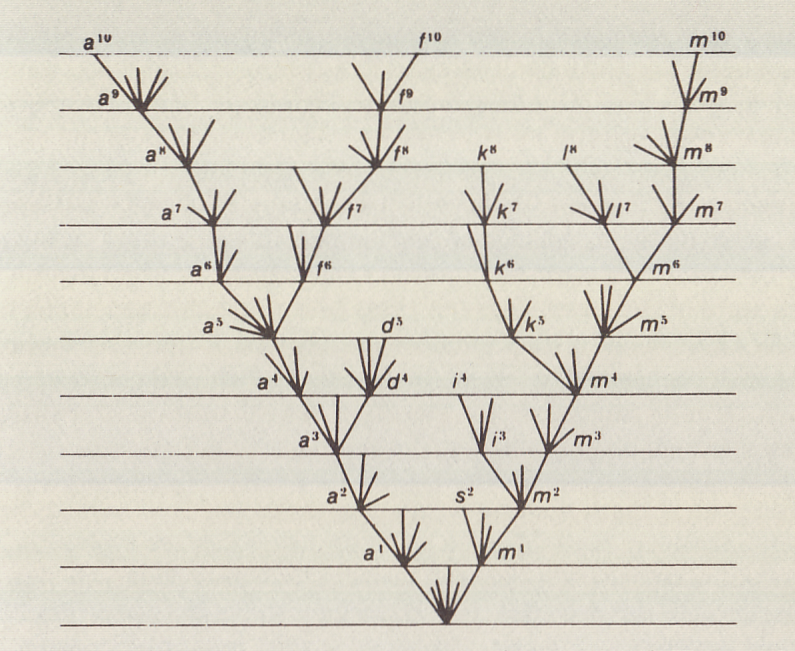
\includegraphics[width=\columnwidth]{./fig/introduction/darwin_origin.png}
\caption[Charles Darwin's Tree]{The only figure in Darwin's Origin of Species.}
\label{fig:darwin_origin}
\end{figure}

\begin{figure}
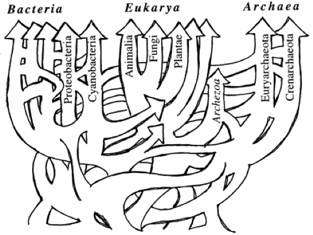
\includegraphics[width=\columnwidth]{./fig/introduction/doolittle_tree.png}
\caption[Ford Doolittle's Tree]{W Ford Doolittle's representation of the universal tree of life with nonvertical evolution.}
\label{fig:doolittle_tree}
\end{figure}

In this thesis, we propose the use of new computational techniques, borrowed from the field of algebraiac topology, to capture and represent complex patterns of genetic exchange that may be obscured using current phylogenetic approaches and tree-centered thinking.

While this may appear obscure at first glance, let us unpack the idea.
Topology is concerned with invariant properties of spaces.
The paradigmatic example is the circle.
Algebraic topology assigns algebraic quantities to these properties and lets us speak and compare spaces quantitatively.

Consider again Darwin's branching phylogeny in Figure \ref{fig:darwin_origin}.
Consider Doolittle's net of life.
Much more complicated topological space.
If we envision these relationships as a topological space, we could use a similar characterization.
The tree is trivially compactable.

there are complications that must be addressed at the outset.
First, deep evolutionary history consists of extinct organisms.
[By the way, how old is life? Mention that.]
Second, we do not have complete sampling.
Third, not all organisms have compatible gene sets to make comparisons.
This is of course why Woese focused on conserved ribosomal RNA, some of the oldest genomic information.

\begin{figure}
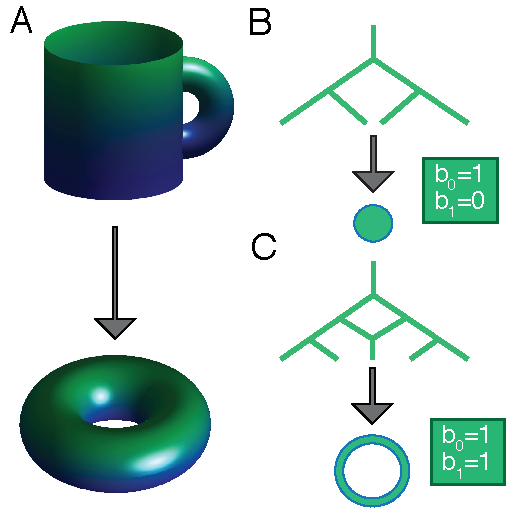
\includegraphics[width=\columnwidth]{./fig/introduction/topology_example.pdf}
\caption[The Paradigmatic Topology Example]{The coffee cup is not trivially contractible. The tree is contractible. The network is not contractible. Betti numbers quantitatively capture these notuons of shape.}
\label{fig:topology_example}
\end{figure}

In this thesis, we use new computational techniques, borrowed from the field of algebraic topology, to capture and represent complex patterns of gene exchange that are obscurbed in current phylogenetic methods.
By doing so, we provide a fuller understanding of evolutionary relationships than allowed by current phylogenetic methods.
Genomic exchange can be characterized by the parental sequences involved in the exchange, by the amount and identity of material exchanged (i.e., the genes or loci involved), and the frequency with which similar exchanges occur.
Techniques such as phylogenetic networks and ancestral recombination graphs have been developed to describe reticulate evolution, but they have had only limited success due to difficulties of biological interpretation and computational infeasibility in all but the smallest datasets.

Should I give a simple description of constructing additive trees

Linkage-based techniques have succeeded in measuring rates of recombination in medium-sized datasets (< 200 sequences), but they cannot reveal the scale of these exchanges (i.e., the genetic distance between parental sequences), and they have limited resolution in pinpointing where along a genome such exchanges have occurred.
A new mathematical foundation is needed to break free of these limitations.

Genome evolution is an extremely rich subject [cite Genome Architecture book].

This thesis contains results of applying methods from topological data analysis to various problems in genomics and evolution.
It primarily details the use of persistent homology as a tool to measure the prevalence and scale of nonvertical evolutionary events, such as reassortments and recombinations.
In so doing, various techniques are developed to extract statistical information from the topological complexes that are constructed.

\subsection{Thesis Organization}

The remainder of this thesis is organized as follows.

In Chapter \ref{ch:background} we present background information on the wide range of topics discussed in this thesis.
This discussion is chiefly structured into two pieces: (1) background on phylogenetics and population genetics, and (2) background on algebraic topology and the methods of topological data analysis.

In Part \ref{part:theory}, we develop two complementary approaches for analyzing genomic data using topological data analysis.
In Chapter \ref{ch:parametric_inference}, we develop methods for performing statistical inference using summary statistics contained in the persistence diagram.
This is the first such use of persistence diagrams as a tool for performing parametric inference.
In Chapter \ref{ch:complex_construction}, we propose alternative methods of constructing topological complexes that generalize the traditional Vietoris-Rips and \Cech complexes but are suited to the particular demands of phylogenetic applications.
We draw on previous work in phylogenetic networks and use homology theory to provide quantitative assessment of reticulation.

In Part \ref{part:application_microorganism} we apply our approach 
In this section, we consider two models.

In Part \ref{part:applications_human}, we apply our approaches to a several problems in human population genetics and biology.
In Chapter \ref{ch:human_recombination_rate} we measure the human recombination rate.
In Chapter \ref{ch:human_population_structre} we reconstruct models of human demographic movements.
In Chapter \ref{ch:human_chromatin_folding} we analyze Hi-C data to understand patterns of chromatin folding in the nucleus.

Finally, in Chapter \ref{ch:conclusions} we summarize our results and present possible avenues for future directions.